\documentclass[10pt]{article}
\makeatletter
\usepackage[autolinebreaks,useliterate]{mcode}
\usepackage{textcomp}
\usepackage{verbatim}
\usepackage{lmodern}
\usepackage{comment}
\excludecomment{Answ}
\usepackage{listings}
\usepackage{color} %red, green, blue, yellow, cyan, magenta, black, white
\definecolor{mygreen}{RGB}{28,172,0} % color values Red, Green, Blue
\definecolor{mylilas}{RGB}{170,55,241}
\renewcommand\paragraph{\@startsection{paragraph}{4}{\z@}%
            {-2.5ex\@plus -1ex \@minus -.25ex}%
            {1.25ex \@plus .25ex}%
            {\normalfont\normalsize\bfseries}}
\makeatother
\usepackage{gensymb}
\setcounter{secnumdepth}{4}
\usepackage{amsmath}
%\usepackage{mathtools}
\usepackage{graphicx}
\usepackage{slashed}
\usepackage{lineno}
\usepackage{latexsym}
\usepackage{subfigure}
\usepackage{amssymb}
\newtheorem{thm}{Theorem}[section]
\newtheorem{cor}[thm]{Corollary}
\newtheorem{lem}[thm]{Lemma}
\usepackage[numbers,sort]{natbib}
\usepackage{enumerate}
\newcommand{\bb}{\begin{equation}}
\newcommand{\ee}{\end{equation}}
\newtheorem{defin}{Definition}
\usepackage{multirow}
\usepackage{ctable}
\usepackage{bm}
\usepackage{enumerate}
\newcommand{\D}[2]{\frac{\partial #1}{\partial #2}}
\newcommand{\DD}[2]{\frac{\partial^2 #1}{\partial #2^2}}
\newcommand{\rd}{\text{ d}}
\newcommand{\disk}{}
\usepackage{framed}
\newcommand{\see}[1]{(see Figure \ref{#1})}
\newcommand{\fig}[1]{Figure \ref{#1}}
\newcommand{\figs}[2]{figures \ref{#1} and \ref{#2}}
\newcommand{\sect}[1]{Section \ref{#1}}
\newcommand{\app}[1]{Appendix \ref{#1}}
\newcommand{\chap}[1]{Chapter \ref{#1}}
\newcommand{\eqn}[1]{equation \eqref{#1}}
\newcommand{\eqns}[2]{equations \eqref{#1} and \eqref{#2}}
\newcommand{\eqnto}[2]{equations \eqref{#1}-\eqref{#2}}
%\usepackage{authblk}
\usepackage{url}
\usepackage{hyperref}
\usepackage{soul}
\newcommand{\eg}{\emph{e.g.} }
\newcommand{\bn}{\bm{n}}
\newcommand{\bu}{\bm{u}}
\newcommand{\ie}{\emph{i.e.} }
\newcommand{\Chapter}[1]{\chapter{#1}\label{#1}}
\newcommand{\Section}[1]{\section{#1}\label{#1}}
\newcommand{\Subsection}[1]{\subsection{#1}\label{#1}}
\newcommand{\Subsubsection}[1]{\subsubsection{#1}\label{#1}}
\newcommand{\Appendix}[1]{\appendix{#1}\label{#1}}
\usepackage[margin=1.5cm,centering]{geometry}
\usepackage[geometry]{ifsym}
\makeatletter
\newcommand\restr[2]{{% we make the whole thing an ordinary symbol
  \left.\kern-\nulldelimiterspace % automatically resize the bar with \right
  #1 % the function
  \vphantom{\big|} % pretend it's a little taller at normal size
  \right|_{#2} % this is the delimiter
  }}
\def\url@leostyle{%
  \@ifundefined{selectfont}{\def\UrlFont{\sf}}{\def\UrlFont{\small\ttfamily}}}
\makeatother
\urlstyle{leo}
\usepackage{multirow}
\usepackage{blkarray}
\usepackage{soul}
\usepackage{framed}
\usepackage{color}
\usepackage{setspace}
\newcommand{\ttttp}{.24\textwidth}
\newcommand{\tttp}{.32\textwidth}
\newcommand{\ttp}{.45\textwidth}
\newcommand{\tbo}{.6\textwidth}
 \usepackage[T1]{fontenc}
\usepackage[utf8]{inputenc}
\usepackage{authblk}
 \renewcommand{\l}{\left(}
\renewcommand{\r}{\right)}
%\begin{figure}[h!!!tb]
%\centering
%\subfigure[\label{Godzilla}]{\includegraphics[height=0.35\textwidth]{./Pictures/Godzilla_final_bw.png}}
%\subfigure[\label{Jaeger}]{\includegraphics[height=0.35\textwidth]{./Pictures/Jaeger_finish_bw.png}}
%\caption{\label{Monsters} The two types of monster we are going to consider are: (a) the naturally occurring Kaijus and (b) the man-made Jaegers.}
%\end{figure}


\begin{document}

\lstset{language=Matlab,%
    %basicstyle=\color{red},
    breaklines=true,%
    morekeywords={matlab2tikz},
    keywordstyle=\color{blue},%
    morekeywords=[2]{1}, keywordstyle=[2]{\color{black}},
    identifierstyle=\color{black},%
    stringstyle=\color{mylilas},
    commentstyle=\color{mygreen},%
    showstringspaces=false,%without this there will be a symbol in the places where there is a space
    numbers=left,%
    numberstyle={\tiny \color{black}},% size of the numbers
    numbersep=9pt, % this defines how far the numbers are from the text
    emph=[1]{for,end,break},emphstyle=[1]\color{red}, %some words to emphasise
    %emph=[2]{word1,word2}, emphstyle=[2]{style},    
}


\title{Problem sheet 1}
\author{Thomas E. Woolley\\Last edited on:}
\maketitle
\section{Early warfare}\label{Early warfare}
Originally\footnote{This question is an adapted version of \href{https://en.wikipedia.org/wiki/Lanchester's_laws}{Lanchester's Laws}. Have a look into how modern warfare differs from early warfare.}, warfare was conducted through hand to hand combat. Thus, a single person had the ability to despatch only one other person at a time. Namely, the combat was \textit{one on one} until one person was unable to fight any longer. Consider two opposing armies of size $A(t)$ and $B(t)$ and suppose $A(0)=A_0$, $B(0)=B_0$, where $A_0>B_0$.
\begin{enumerate}

\item Suppose the armies are equally matched such that when members of the $A$ and $B$ armies meet they are both equally like to win the fight. Further, assume that the interaction rate constant between the two armies is $r$, write the above combat interaction down as two interaction equations.

\item Show that the Law of Mass Action can be used to convert the early warfare interactions into the following ODEs,
\begin{align}
\dot{A}=-rAB,\quad A(0)=A_0,\label{A}\\
\dot{B}=-rAB,\quad B(0)=B_0.\label{B}
\end{align}

\item \label{Stst}Derive the steady states of \eqns{A}{B}. What happens when you try to characterise their stability?

\item Show that
\bb
A(t)=B(t)+\textrm{Constant},\label{Constant}
\ee
where you should define the constant explicitly.

\item In question \ref{Stst} you should have found that there was an infinite number of steady states. Show how \eqn{Constant} collapses all possibilities to just one.

\item Construct the $(A,B)$ phase plane and use it to characterise the steady states stability.\label{Ppq}

\item Show that \eqns{A}{B} can be rewritten as
\begin{align}
\dot{A}=-rA(A-A_0+B_0),\label{AA}\\
\dot{B}=-rB(B+A_0-B_0).\label{BB}
\end{align}

\item Derive the steady states of \eqns{AA}{BB}.

\item Considering \eqns{AA}{BB} as separate scalar ODEs characterise the stability of the previously derived steady states analytically and graphically through constructing the phase planes $\l A,\dot{A} \r$ and $\l B,\dot{B}\r$.\label{Scalar}

\item Consider \eqns{AA}{BB} as a system and characterise the stability of the steady states algebraically and graphically by plotting the $(A,B)$ phase plane.\label{System}

\item Do the results from questions \eqref{Scalar} and \eqref{System} correspond to the results from question \ref{Ppq}?

\item Solve \eqns{AA}{BB} explicitly and sketch the resulting $(t,A(t))$ and $(t,B(t))$ curves on the same axis.

\item You have now derived the same result in three different ways. Without referring to the mathematics, interpret your result.
\end{enumerate}
\begin{Answ}
\subsection{Answers}
\begin{enumerate}
\item Since combat is one on one then one person from the $A$ side will interact with one person from the $B$ side, thus, the interaction term is $A+B$. Since the fight happens until one of the combatants can no longer compete there are two possible outcomes, either $A$ wins or $B$ wins. Thus the two interaction equations are
\begin{align}
A+B\stackrel{r}{\rightarrow}A,\label{Interaction_A}\\
A+B\stackrel{r}{\rightarrow}B.\label{Interaction_B}
\end{align}

\item Equations \eqref{A} and \eqref{B} follow directly from applying the Law of Mass Action to \eqns{Interaction_A}{Interaction_B}.

\item There are two infinite families of steady states, of the form $\l \hat{A},0 \r$ and $\l 0,\hat{B}\r$ for any constant values $\hat{A}$, or $\hat{B}$. The Jacobian of the system is
\bb
J=\left[ \begin{array}{cc} -rB&-rA\\
-rB&-rA
\end {array} \right],
\ee
and
\bb
J(\hat{A},0)=\left[ \begin{array}{cc} 0&-r\hat{A}\\
0&-r\hat{A}
\end {array} \right],\quad J(0,\hat{B})=\left[ \begin{array}{cc} -r\hat{B}&0\\
-r\hat{B}&0
\end {array} \right].
\ee
In both cases one eigenvalue is negative and the other is zero. Thus, the linear analysis is inconclusive.

\item Subtracting \eqn{B} from \eqn{A} provides
\bb
\dot{A}-\dot{B}=0.\label{A-B}
\ee
Integrating both sides of \eqn{A-B} with respect to time provides
\bb
\int^t_0\frac{\rd}{\rd t'}(A-B)dt'=0,
\ee
which upon simplification and rearranging is
\bb
A(t)=B(t)-B_0+A_0.\label{Constant_answer}
\ee

\item Question \ref{Stst} led us to derive that $\l \hat{A},0 \r$ and $\l 0,\hat{B}\r$ are steady states for all constant values of $\hat{A}$ and $\hat{B}$. However, we also have to satisfy \eqn{Constant_answer}. Since $A_0>B_0$ we must have that $\lim_{t\rightarrow\infty} B(t)=0$ and $\lim_{t\rightarrow\infty} A(t)=\hat{A}=A_0-B_0$.


\item The $(A,B)$ phase plane is given in \fig{PPAB1}. We observe that the horizontal and vertical axes are the nullclines and the steady states. Further, in the positive $(A,B)$ quadrant both $A$ and $B$ are decreasing. However, the trajectories must travel along a line of $B=A-$Constant as derived earlier. The initial conditions pick exactly one of these lines and the trajectory heads to $\l 0,\hat{A} \r$ as derived. Since we must remain on this line and the populations cannot go negative $\l 0,\hat{A}\r$ is stable.
\begin{figure}[h!!!tb]
\centering
\includegraphics[width=\ttp]{../../Pictures/PPAB1}
\caption{\label{PPAB1} $(A,B)$ phase plane of \eqns{A}{B}.}
\end{figure}

\item Substituting \eqn{Constant_answer} into \eqns{A}{B} gives \eqns{AA}{BB}.
\item  The steady states are $(0,0)$, $(0,B_0-A_0)$, $(A_0-B_0,0)$ and $(A_0-B_0,B_0-A_0)$.

\item We first note that $A_0-B_0>0$. From the last question the steady states of 
\bb
\dot{A}=-rA(A-A_0+B_0)=f(A)
\ee
are  $A_{st}=0,A_0-B_0$. Deriving
\bb
f'(A)=-2rA-r(B_0-A_0)
\ee
and substituting in the steady states give
\begin{align}
f'(0)=-r(B_0-A_0)>0,\\
f'(A_0-B_0)=-r(A_0-B_0)<0.
\end{align}
Thus, $A_{st}=0$ is unstable and $A_{st}=A_0-B_0$ is stable.

Similarly, if $g(B)=-rB(B+A_0-B_0)$ and the steady states are $B_{st}=0, B_0-A_0$ then
\bb
g'(B)=-2rB-r(A_0-B_0)
\ee
and
\begin{align}
g'(0)=-r(A_0-B_0)<0\\
g'(B_0-A_0)=-r(B_0-A_0)>0.
\end{align}
Thus, $B_{st}=0$ is stable and $B_{st}=B_0-A_0$ is unstable. Also note $B_{st}=B_0-A_0<0$, which is unphysical and so we do not really need to consider it.

The phase planes of $\l A,\dot{A}\r$ and $\l B,\dot{B}\r$ are shown in \fig{PP2}
\begin{figure}[h!!!tb]
\centering
\subfigure[\label{PPA1}]{\includegraphics[width=\ttp]{../../Pictures/PPA1.png}}
\subfigure[\label{PPA2}]{\includegraphics[width=\ttp]{../../Pictures/PPA2.png}}
\caption{\label{PP2} Phase planes of \eqns{AA}{BB}.}
\end{figure}

\item The Jacobian of \eqns{AA}{BB} is
\bb
J_2=\left[ \begin{array}{cc}-2rA-r(B_0-A_0)&0\\
0&-2rB-r(A_0-B_0)
\end {array} \right],
\ee
and, so,
\begin{itemize}
\item the eigenvalues of $J_2(0,0)$ are $\lambda_{1,2}= \pm r(B_0-A_0)$, thus, $(0,0)$ is a saddle point;
\item the eigenvalues of $J_2(A_0-B_0,0)$ are $\lambda_{1,2}= -r(A_0-B_0)<0$, thus, $(A_0-B_0,0)$ is a stable node;
\item  the eigenvalues of $J_2(0,B_0-A_0)$ are $\lambda_{1,2}= -r(B_0-A_0)>0$, thus, $(0,B_0-A_0,0)$ is an unstable node;
\item  the eigenvalues of $J_2(A_0-B_0,B_0-A_0)$ are $\lambda_{1,2}= \pm r(A_0-B_0)$, thus, $(A_0-B_0,B_0-A_0)$ is a saddle point.
\end{itemize} 
The accompanying phase plane is shown in \fig{PPAB2}.
\begin{figure}[h!!!tb]
\centering
\includegraphics[width=\ttp]{../../Pictures/PPAB2.png}
\caption{\label{PPAB2} Phase plane of \eqns{AA}{BB}.}
\end{figure}


\item When we analysed system \eqref{A}-\eqref{B} initially we found that the linear analysis approach did not work. However, converting system \eqref{A}-\eqref{B}
to system \eqref{AA}-\eqref{BB} does allow us to use the algebraic techniques. However, converting from \eqref{A}-\eqref{B} to system \eqref{AA}-\eqref{BB} does introduce a number of ``artificial'' steady states. However, these are all unstable and in all cases we reproduce that the system tends to $(0,A_0-B_0)$.

\item Let us, first,  solve \eqn{AA}. Using partial fractions we get that \eqn{AA} is equivalent to
\begin{align}
\int^{A(t)}_{A_0}-\frac{1}{\l A_0-B_0 \r A}+\frac{1}{
 \l A_0-B_0\r  \l A- A_0+B_0
 \r }=&\int^{t}_{0}-r\rd t',\\
 \implies -\frac{1}{\l A_0-B_0 \r}\left[\ln(A)\right]^{A(t)}_{A_0}+\frac{1}{\l A_0-B_0 \r}\left[\ln(A-A_0+B_0)\right]^{A(t)}_{A_0}=&-rt,\\
 \implies -\ln\l \frac{A(t)}{A_0}\r+\ln\l \frac{A(t)-A_0+B_0}{B_0}\ \r=&-(A_0-B_0)rt,\\
  \implies \frac{\l A(t)-A_0+B_0\r A_0}{B_0A(t)}=&\exp(-(A_0-B_0)rt),\\
    \implies 1-\frac{\l A_0-B_0\r }{A(t)}=&\frac{B_0}{A_0}\exp\l -(A_0-B_0)rt\r,\\
    \implies A(t)=&\frac{\l A_0-B_0\r }{1-\frac{B_0}{A_0}\exp\l -(A_0-B_0)rt\r}.\label{At}
\end{align}
$B(t)$ can then simply be obtained from \eqn{Constant_answer},
\begin{align}
B(t)=&A(t)+B_0-A_0,\\
=&\frac{\l A_0-B_0\r }{1-\frac{B_0}{A_0}\exp\l -(A_0-B_0)rt\r}+B_0-A_0,\\
=&(A_0-B_0)\l\frac{1}{1-\frac{B_0}{A_0}\exp\l -(A_0-B_0)rt\r}-1\r,\\
=&(A_0-B_0)\l \frac{ B_0 \exp\l -(A_0-B_0)rt\r }{ A_0-B_0 \exp\l -(A_0-B_0)rt\r }\r.\label{Bt}
\end{align}
Considering \eqns{At}{Bt} we see that $A(0)=A_0$, $B(0)=B_0$, as required and that $A(t)\rightarrow A_0-B_0$, $B(t)\rightarrow 0$ as $t\rightarrow \infty$. A sketch of $A(t)$ and $B(t)$ can be found in \fig{AB_sketch}.
\begin{figure}[h!!!tb]
\centering
\includegraphics[width=\ttp]{../../Pictures/AB_sketch.png}
\caption{\label{AB_sketch} Solutions of \eqns{AA}{BB}.}
\end{figure}
\item Early warfare was simply a numbers game. The largest army would win, with losses equal to the size of the other army. Essentially, you were trading lives one for one. Captain America would not be pleased.

\end{enumerate}
\end{Answ}

\section{Non-dimensionalisation and interpretation}
Consider the following set of interaction equations for two animal populations $N$ and $P$.
\begin{align}
&\frac{\rd N}{\rd t} =rN\l 1- \frac{N}{K}\r-bNP,\label{N}\\
&\frac{\rd P}{\rd t} =ebNP-mP.\label{P}
\end{align}
where $b, e, K, r$ and $m$ are positive constants and the initial conditions are $N_0$ and $P_0$, respectively.
\begin{enumerate}
\item What type of interaction is occurring between $N$ and $P$?
\item Write down a set of interaction equations that could give rise to \eqns{N}{P}.
\item Non-dimensionalise \eqns{N}{P} to get the form
\begin{align}
&\frac{\rd u}{\rd \tau} =c_1u\l 1- u\r-uv,\label{u}\\
&\frac{\rd v}{\rd \tau} =c_2uv-v,\label{v}
\end{align}
where $c_1$ and $c_2$ should be defined explicitly in terms of $K, b, e, r$ and $m$.
\item Provide an interpretation of $c_1$ and $c_2$.
\item Suppose the predator is a pest and we want to wipe the predator out, whilst maintaining a positive prey population (\eg consider a fox and hen scenario). What strategy best achieves this, in terms of altering the sizes of $c_1$ and $c_2$? Explicitly, is it best to:
\begin{itemize}
\item increase $c_1$?
\item increase $c_2$?
\item increase both?
\item decrease $c_1$?
\item decrease $c_2$?
\item decrease both?
\item increase $c_1$ and decrease $c_2$?
\item decrease $c_1$ and increase $c_2$?
\end{itemize} 
Explain your choice.
\item Having chosen a strategy consider how best to enact the changes of $c_1$ and/or $c_2$ in terms of altering $b, e, K, r$ and $m$. What are the pros and cons? What would your advice be of best strategy?
\end{enumerate}





\begin{Answ}
\subsection{Answers}
\begin{enumerate}
\item $N$ and $P$ are undergoing a predator-prey reaction, with $N$ as the prey and $P$ as the predator. This is because whenever $N$ and $P$ interact through the $NP$ term the $N$ population decreases, whilst the $P$ population increases. In the absence of predator, $N$ will manage its population logistically, whilst in the absence of prey, $P$ will die out.
\item Note the following are not unique, so if you have a variation on those below, as long as they still work that is fine.
\begin{align}
N&\mathrel{\mathop{\rightleftarrows}^{r}_{r/K}}N+N,\\
P&\stackrel{m}{\rightarrow}\slashed{0},\\
N+P&\stackrel{b}{\rightarrow}(1+e)P.
\end{align}
\item Let $N=[N]u, P=[P]v$ and $t=[t]\tau$. Where $u,v$ and $\tau$ are non-dimensional and $[N]$, $[P]$ and $[t]$ are dimensional constants. Substituting these into \eqns{N}{P} we derive
\begin{align}
\frac{[N]}{[t]}\frac{\rd u}{\rd \tau} =&r[N]u\l 1- \frac{[N]u}{K}\r-b[N][P]uv,\label{NondimN}\\
\frac{[P]}{[t]}\frac{\rd v}{\rd \tau} =&eb[N][P]uv-m[P]v.\label{NondimP}
\end{align}
Rearranging we get
\begin{align}
\frac{\rd u}{\rd \tau} =&[t]ru\l 1- \frac{u[N]}{K}\r-b[t][P]uv,\label{Nondimu}\\
\frac{\rd v}{\rd \tau} =&eb[N][t]uv-m[t]v.\label{Nondimv}
\end{align}
Comparing \eqns{Nondimu}{Nondimv} to \eqns{u}{v} we see that we want to fix $[N]=K$, $[t]=1/m$ and $[P]=1/(b[t])=m/b$. From these we can see that $c_1=[t]r=r/m$ and $c_2=eb[N][t]=ebK/m$.
\item Since $m$ is the predator death rate and $r$ is the reproduction time scale $c_1=r/m$ is, thus, non-dimensional as it is a ratio of time-scales. Critically, it measures the system's robustness to change. For example, if $c_1$ is very large then $r$ is very large (meaning a high birth rate), or $m$ is very small (low death rate). In this case perturbations to the systems will have small effects. Alternatively is $c_1$ is small (\ie small birth rate, or large death rate) the system is much more fragile to interference.

$eb$ is the gain of predator from every predator-prey interaction, $m$ is predator death rate, thus, $eb/m$ is a net measure of how many predators are gained in every interaction.  $K$ is carrying capacity of the domain, \ie the maximum number of prey. Thus $c_2=eb/m \times K$ is the \textit{maximum predator fecundity}, it is a measure of how large the predator population can be.
\item Considering the interpretations of $c_1$ and $c_2$ from the previous question we see that to reduce the predator population we want to reduce $c_2$. Altering $c_1$ simply changes the time scale on which the alterations happen.

\item Since $c_2=ebK/m$ then to reduce the predator population we can either decrease $e$, $b$, or $K$, or increase $m$. Critically, reducing $K$ would reduce the carrying capacity of the prey, which we do not want to do. Thus, we are left with altering $e$, $b$, or $m$. Considering each of these in turn,
\begin{itemize}
\item decreasing $e$ represents reducing the ability of the predator to turn food into reproduction. One unlikely way of achieving this is reduce the nutritional value of the prey. Not only would this be difficult, but it will probably also reduce the profitability of our prey stock. An alternative and more widely used way is releasing sterilised predators into the wild. Although the predators will continue to pre-date, they will not be able to reproduce and, thus, we can drive the predators to extinction. However, this is often a slow and costly strategy.
\item decreasing $b$ represents reducing predation encounters. Thus, we could increase security around the prey, essentially isolating them from attack. This is one reason why battery farming is cheaper, namely fewer chickens are lost to wild animal attacks. This is often a cheaper strategy than above, but we have to question the humanity of isolating the animal from its natural habitat.
\item increasing $m$ represents killing the predator, perhaps through poison, or active predator hunting. Again, we have to question the humanity of this option as well as the cost-benefit when compared with decreasing $b$.
\end{itemize}
As for best strategy? As long as you have considered some of the above points, and maybe others you can think of, then any defensible position will be based on the specifics of a given case. For example, it is easier to wipe out a pest like termites than it is to wipe out a fox population. Equally, mixed strategies are often the most beneficial, namely, sterilisation alongside culling, alongside prey protection.
\end{enumerate}
\end{Answ}
\section{Using \texttt{ode45}}
As in MA0232 I will be offering you the chance to have a go at understanding Matlab. It is free to download, all you need is follow this (clickable) link \url{https://uk.mathworks.com/academia/tah-support-program/eligibility.html} and sign up using your Cardiff email address.

Throughout this course we will be simulating ODEs of many types and, thus, it is good to be able to check your answers. The more you simulate, the better your intuition. In order to simulate ODEs we are going to use Matlab's inbuilt command \texttt{ode45}. Matlab has several ODE solvers, but  \texttt{ode45} is the most general ``catch all'' code. Essentially, you try it first and if it does not work you try something more specific. However, for our purposes it will be adequate. 

For a high level description of \texttt{ode45} type \texttt{help ode45}, or \texttt{doc ode45} into Matlab and it will bring up a brief description and a full description, respectively. Here, I will provide a brief overview of a general code that will work on most systems throughout this course.

The code below should be available as \verb General_ode45_code.m  and it solves problem \ref{Early warfare}. Either download it directly, or copy and paste it into Matlab. The green text are comments to help you understand what is going on. Essentially, for different ODE systems you should only really have to change the description in lines 49-50. Note you may also need to change the length of time over which the equations are solved (\texttt{Tend}).
\lstset{numbers=none}
\begin{lstlisting}
%% Ensure we start from a blank slate
clear all
close all
clc

%% Initialise variables
fs=15; % Set fontsize

Tend=0.3; % Set final time
N=100; % Set number of steps
t=linspace(0,Tend,N); % Set number of time points at which the solution is to be evaluated
IC=[200;
    190]; %Initial conditions as a column vector

%% Solve ODE

% Each component is a row in the matrix y.
[t,y] = ode45(@ODE_function,t,IC);

%% Plot Solution

%%% (time,solution plots)
hold on % Allows us to plot multiple graphs at once
plot(t,y(:,1)) % Plots the first solution
plot(t,y(:,2)) % Plots the second solution
legend('u','v') % Adds a legend and defines the lines for clarity

% Label axes for clarity
xlabel('t') 
ylabel('Solutions')

set(gca,'fontsize',fs) % Changes the axis fontsize

%%% Phasespace plots
figure % Starts a new figure without overwriting the previous one
plot(y(:,1),y(:,2))
xlabel('u') 
ylabel('v')
set(gca,'fontsize',fs)




%% ODE description
function dydt=ODE_function(t,y)
r=1; %Interaction parameter

% Defining the ODEs as a column vector. Each row is one of the ODEs.
dydt=[-r*y(1)*y(2) %Line 49
      -r*y(1)*y(2)]; %Line 50

end
\end{lstlisting}

Once you have had a play with the above code try and adapt it to solve \eqns{u}{v}.

\section*{Exam Revision}
Problem sheets 3-5 of course MA0232 contain many examples and solutions that will provide adequate practice at: deriving steady states, non-dimensionalisation, characterising stability and sketching graphs.

\end{document}